\chapter{Introduction}\label{ch:introduction}
Congratulations on acquiring an AIDA2020 \gls{tlu}. We hope that the unit will help you to collect lots of useful data during your hardware tests.\\
This manual describes the \gls{tlu} designed for the \href{http://aida2020.web.cern.ch/}{AIDA-2020 project} by David Cussans\footnote{University of Bristol, Particle Physics group} and Paolo Baesso\footnote{University of Bristol, Particle Physics group}.\\
The unit is designed to be used in High Energy Physics beam-tests and provides a simple and flexible interface for fast timing and triggering signals at the AIDA pixel sensor beam-telescope.\\
The current version of the hardware is an evolution of the \href{https://twiki.cern.ch/twiki/bin/view/MimosaTelescope/TLU}{EUDET-TLU} and the \href{https://www.ohwr.org/projects/fmc-mtlu/wiki}{miniTLU} and is shipped in a metal enclosure that includes an \gls{fpga} board, the \gls{tlu} \gls{pcb} and an additional power module: the \gls{fpga} is responsible for all the logic functions of the unit, while the \gls{pcb} contains the clock chip, discriminator and interface blocks needed to communicate with other devices. The power module contains programmable \gls{dac} to power photomultipliers and \gls{led} indicators.\\
The current version of the \gls{pcb} is \brd and is designed to plug onto a carrier \gls{fpga} board like any other \gls{fmc} mezzanine board, although its form factor does not comply with the ANSI-VITA-57-1 standard.\\

\section{Overview}
The AIDA \gls{tlu} provides timing and synchronization signals to test-beam readout hardware.\\
When used for within AIDA-2020 specifications, the hardware generates a low-jitter 40~MHz clock or can accept an external clock reference. The external reference clock frequency is not required to be 40~MHz but other values require a dedicated configuration of the clock circuitry on the board. Similarly, by changing the configuration file it is possible to operate the hardware at different clock frequencies.\\
The \gls{tlu} accepts asynchronous trigger signals from up to six external sources, such as beam-scintillators, and generate synchronous signals (including global trigger or control signals) to send to up to four \gls{dut}. The logic function used to generate the trigger can be defined by the user among all the possible logic combinations of the inputs.\\
Depending on the chosen mode of operation, the \gls{tlu} can accept busy signals or other veto signals from \gls{dut}s and react accordingly, for instance avoiding any further trigger until all the busy signals have been de-asserted.\\
Whenever a global trigger is generated by the unit, a 48-bit coarse time-stamp is attached to it. This time stamp is based on the internal clock. The unit also records a fine-grain time stamp with 780~ps resolution for each signal involved in the trigger decision.\\
The configuration parameters and data are sent and received via the \href{https://www.ohwr.org/projects/ipbus}{IPbus} which provides a simple way to control and communicate TCA-based hardware via the UDP/IP protocol.\\
The \gls{tlu} is shipped with an \gls{fpga} board already programmed with the latest version of the firmware needed to operate the unit. New features and bug fixes are continuously being implemented by the developing team and it is possible to flash the unit with a new firmware as described in section~\ref{ch:flashFPGA}.\\
The unit requires 12~V to operate. Power can be provided using the circular socket located on the back panel. See section~\ref{ch:backpanelintro} for details on compatible connectors.\\
During normal operation the current drawn by the unit is about 1~A.

\section{Front panel}\label{ch:frontpanel}
The front panel of the \gls{tlu} is shown in figure~\ref{fig:frontpanel}; from left to right, the main elements are:
\begin{itemize}
  \item \gls{sfp} cage
  \item 4 \gls{hdmi} connectors for devices under test. Each connector has a \gls{rgb} LED used to indicate the port status (see section~\ref{ch:frontpanelintro}).
  \item 1 LEMO connector for \gls{lvds} clock input/output. This is a 2-pin LEMO series 00 connector\footnote{Part number EPG.00.302.NLN. An example of mating part is LEMO FGG.00.302.CLAD35}. A \gls{rgb} \gls{led} indicator is used to signal whether the port is configured as input or output.
  \item 6 LEMO Trigger inputs. These are standard 1-pin LEMO connectors\footnote{LEMO EPK.00.250.NN. Mates with any LEMO 00.250 connector}. Each input has a \gls{rgb} \gls{led} indicator.
  \item 4 LEMO connectors to provide power to photomultipliers. This is a 4-pin connector with 9-mm diameter\footnote{LEMO part number EXP.0S.304.HLN. Mates with LEMO part FFA.0S.304.CLAC44 or similar.}. For the pin-out see section~\ref{ch:frontpanel}.
  \begin{alertinfo}{Note}
    To reduce the cost of a unit, some modules are not equipped with these connectors and the front panel holes are blanked by a plastic board.\\
    If necessary, it is possible to solder the connectors at a later stage, since all the necessary circuitry is present. This requires disassembling the unit, removing the top cover. See section~\ref{ch:inspection} for details.
  \end{alertinfo}
  \item Green \gls{led} indicators for power (+12 V) and regulators (+5 V and -5 V).
\end{itemize}
\begin{figure}
  \centering
  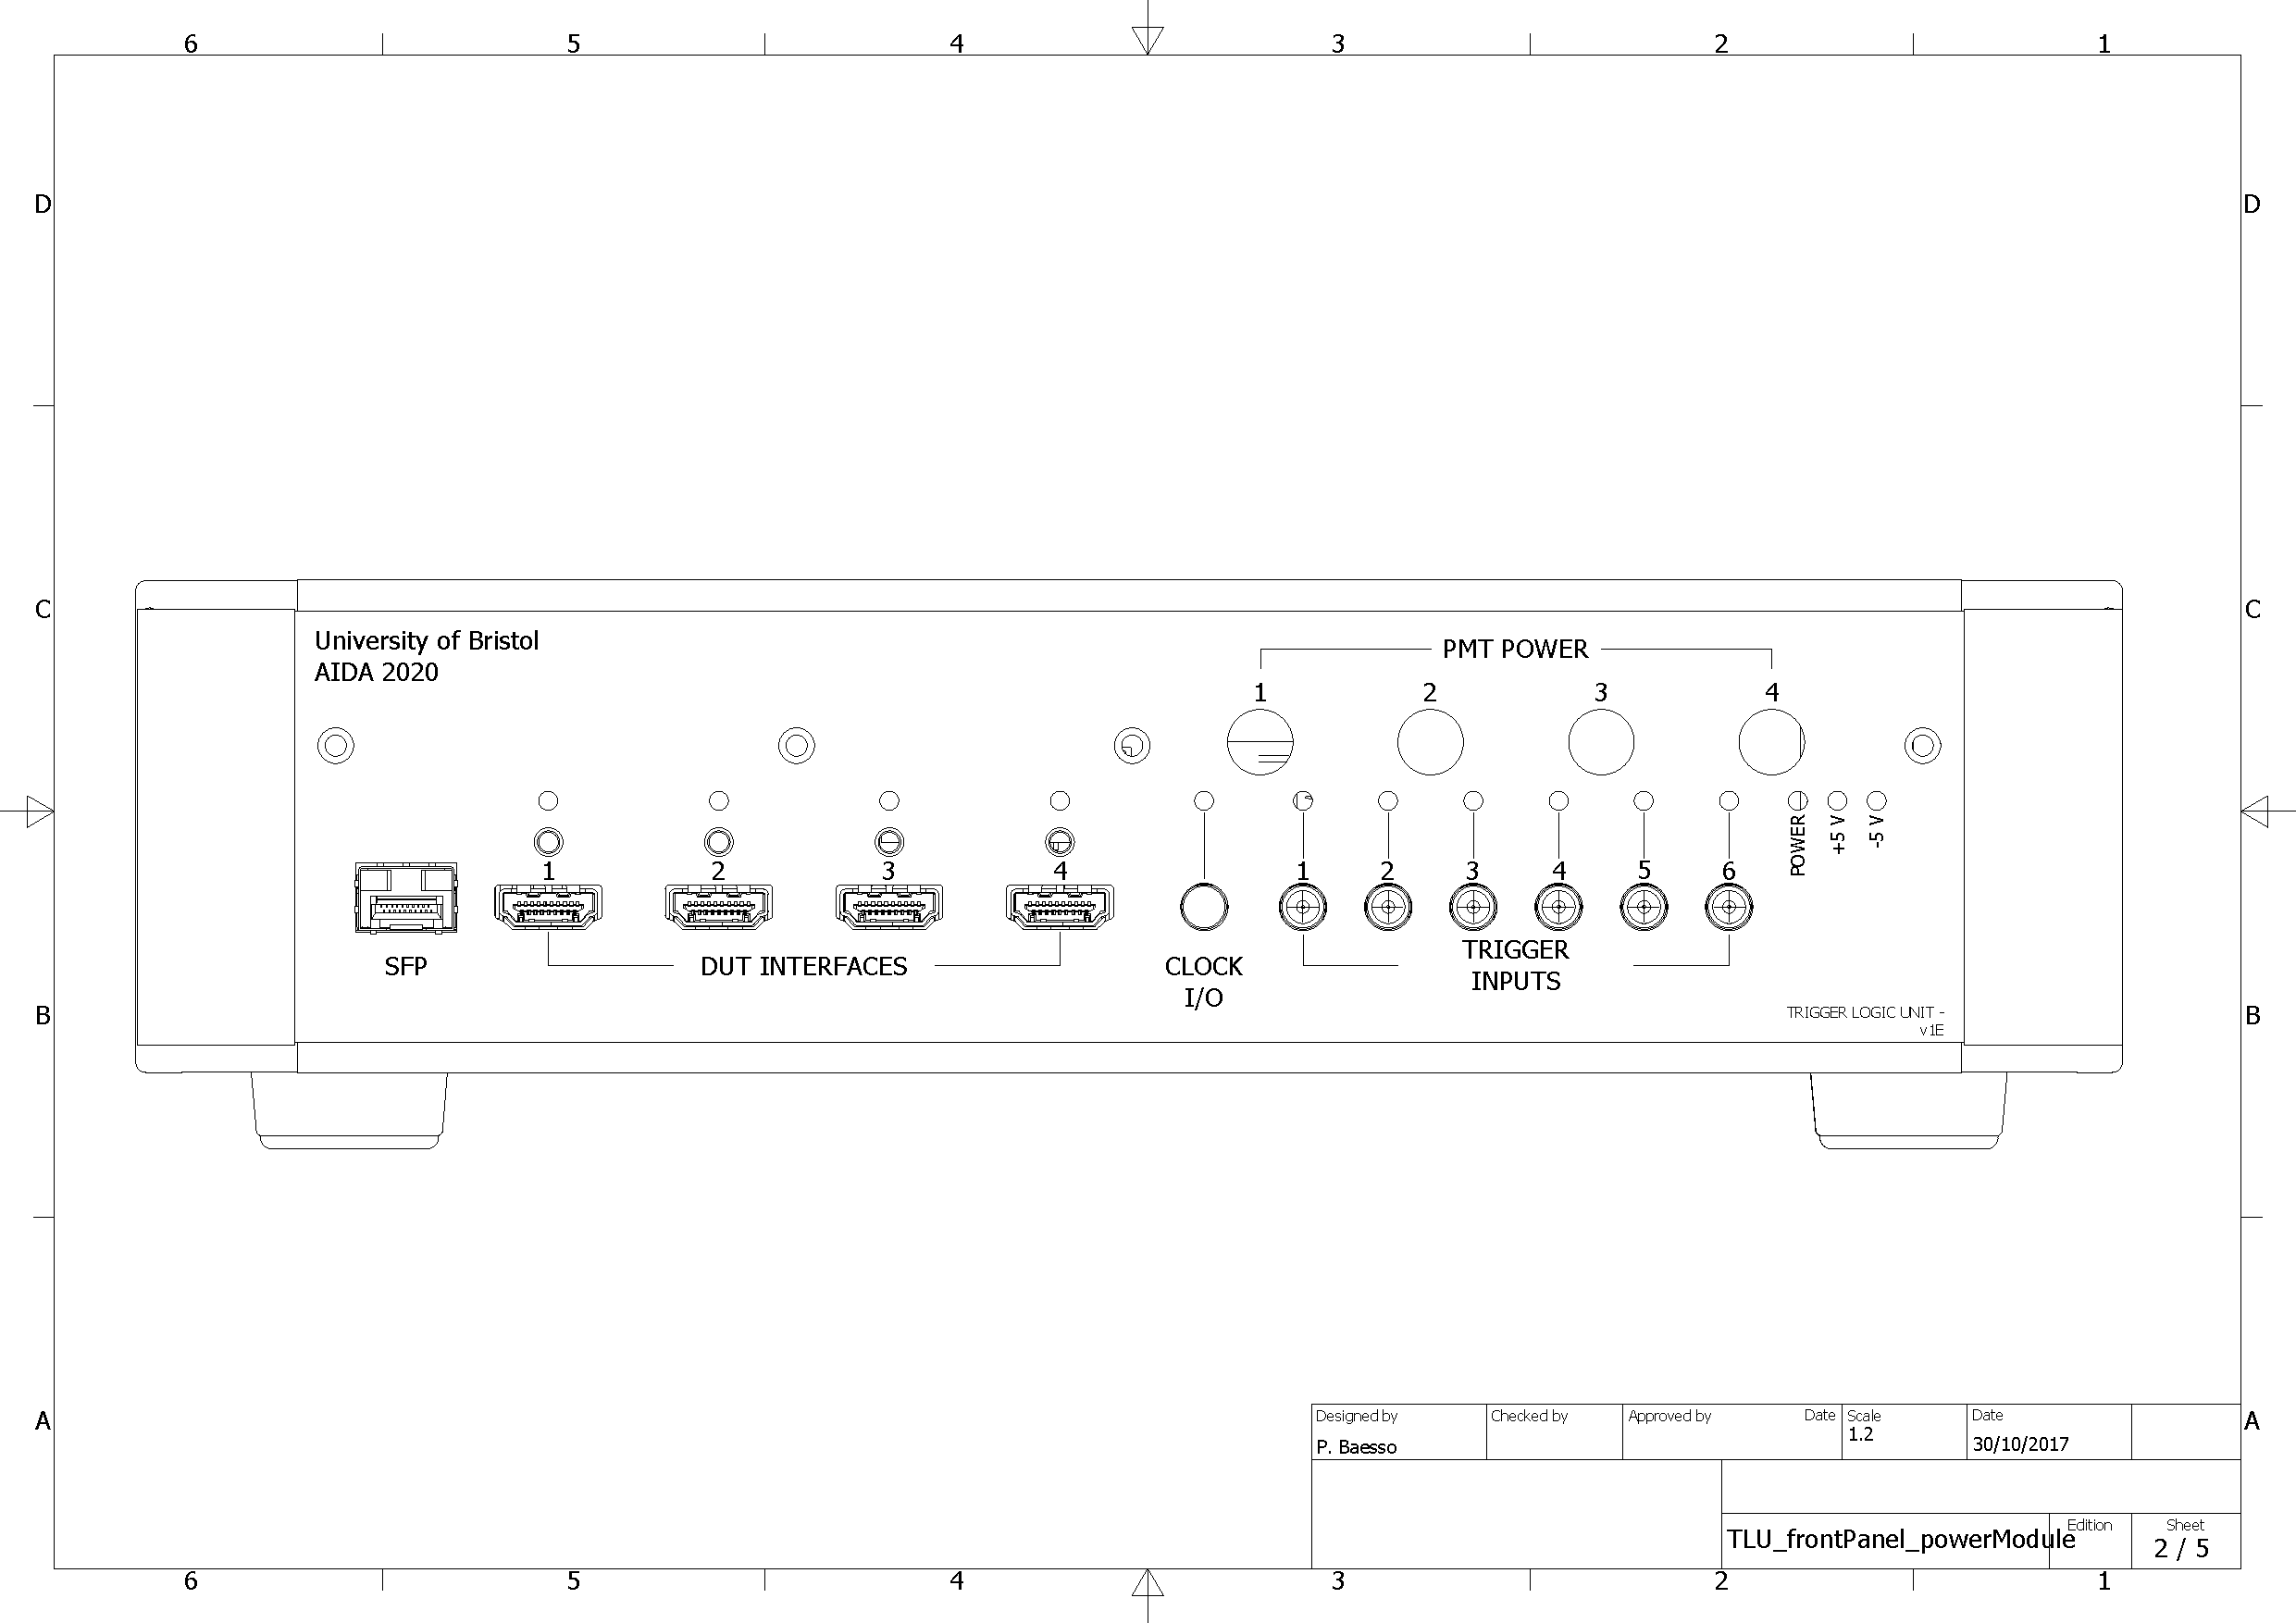
\includegraphics[width=.950\textwidth]{./Images/frontPanel.pdf}
  \caption{View of the TLU front panel.}
  \label{fig:frontpanel}
\end{figure}

\section{Back panel}\label{ch:backpanelintro}
The \gls{tlu} back panel is shown in figure~\ref{fig:backpanel}; from left to right, the main elements are:
\begin{itemize}
  \item RJ45 connector: this is the connector used to communicate with the hardware using IPBus.
  \item \gls{usb}-B port used to flash the internal logic with a new version of the firmware. See section\ref{ch:fpgahardware} for details.
  \begin{alertinfo}{Note}
    This port should be left disconnected if planning to use the self-boot capability of the internal logic. If a cable is detected, the \gls{fpga} will not load the pre-flashed firmware at power-up.
  \end{alertinfo}
  \item \gls{usb}-B port used to communicate with the \gls{fpga} \gls{uart} port.
  \item Power connector\footnote{All TLUs shipped after 17/06/2018 use Switchcraft 721A; mates with a $\phi$~5.5 mm jack with $\phi$~2.5 mm central pin. For instance use Lumberg 1634 02.\\ TLUs shipped before that date use Switchcraft 722A instead, which mates with a $\phi$~5.5 mm jack with $\phi$~2.1 mm central pin. For instance use Lumberg 1633 02. Only 3 units are currently still using the 2.1~mm connector.}. Central pin is +12 V. It is recommended to use a power supply capable of providing at least 1~A.
\end{itemize}
\begin{figure}
  \centering
  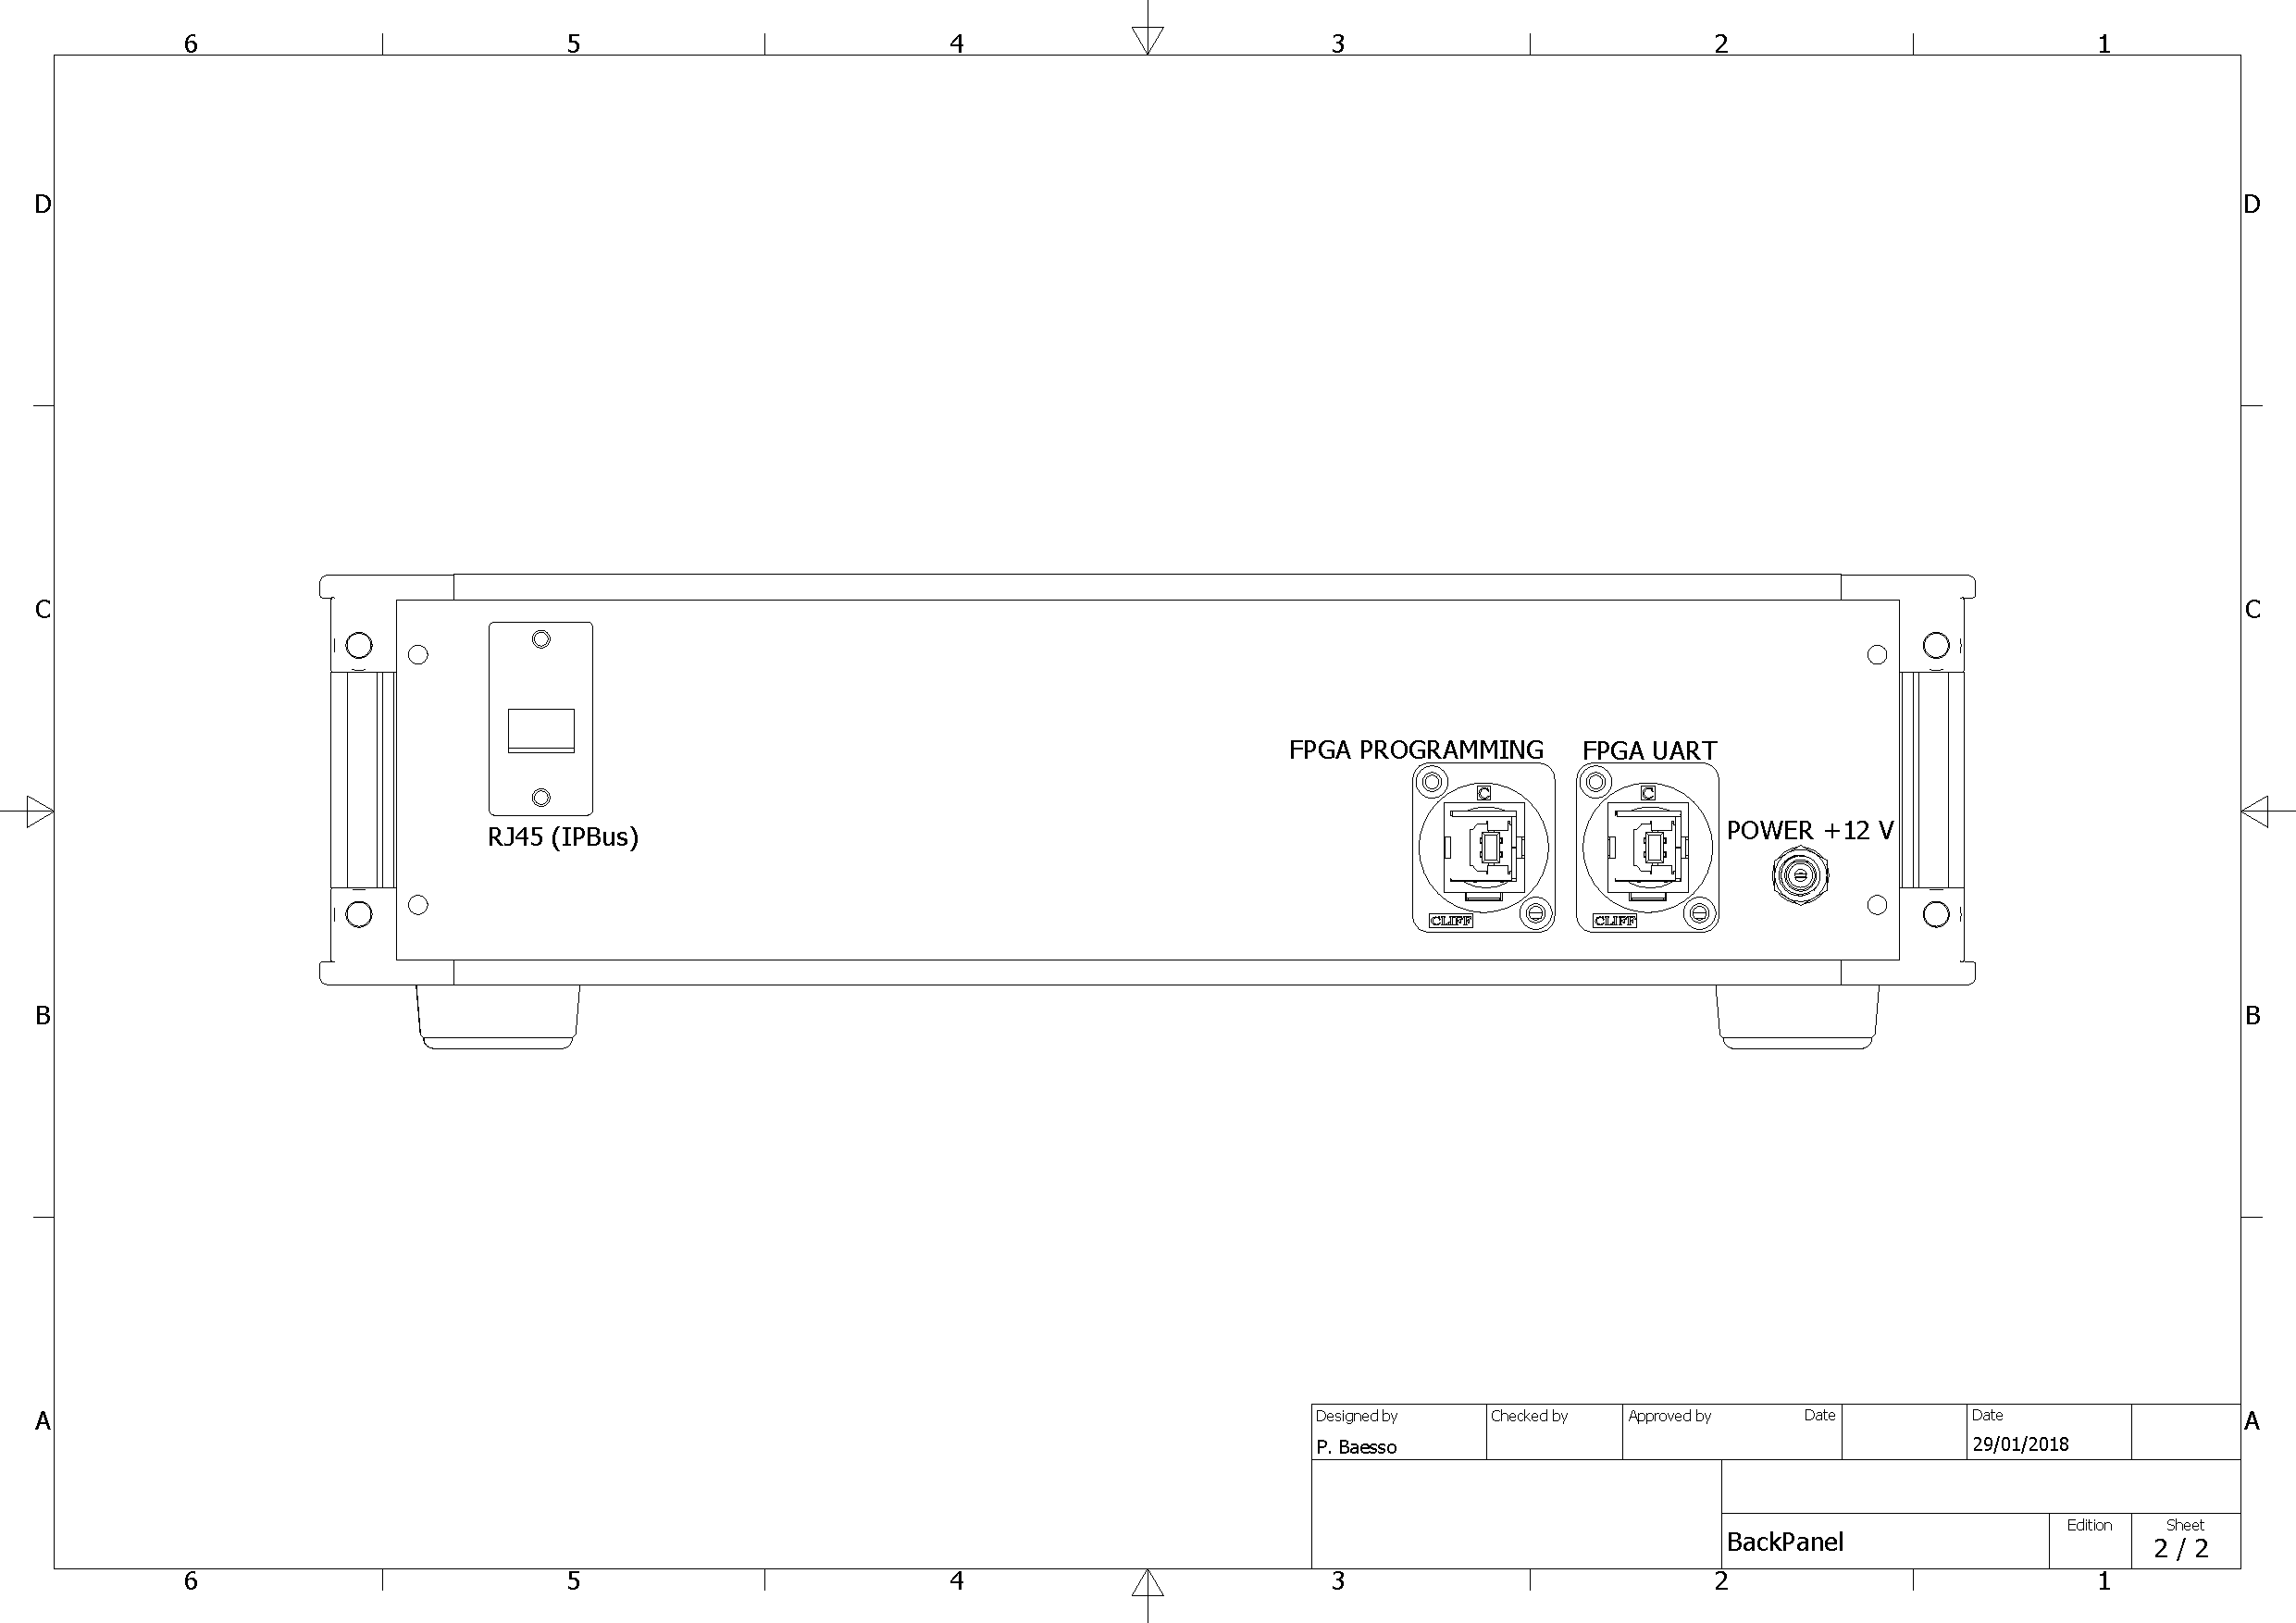
\includegraphics[width=.950\textwidth]{./Images/backPaneldoc.pdf}
  \caption{View of the TLU back panel.}
  \label{fig:backpanel}
\end{figure}
A cooling fan (not shown in figure~\ref{fig:backpanel} is also mounted on the back panel.

\section{Setup}\label{ch:setup}
At the moment of shipping, each \gls{tlu} is pre-configured with the most recent version of the firmware. It is therefore possible to power the unit and start using it almost immediately. The following steps are required to use the unit:
\begin{enumerate}
  \item Ensure no \gls{usb} cable is plugged in the unit
  \item Power the unit using the provided power supply (+12~V) or an equivalent power supply. The pre-configured firmware will automatically load.
  \item Plug an Ethernet cable in the back panel and connect it to the computer used to run the control software. Note that currently the unit uses a pre-defined IP address of 192.168.200.30. In future version of the firmware the address will be configurable.
  \item Use the control software to configure the unit. In particular, after each power up it is necessary to re-configure the clock chip. See chapter~\ref{ch:controlsw} for details on the software and chapter~\ref{ch:clock} for details on the clock chip.
\end{enumerate}

\section{FPGA and firmware}\label{ch:fpgahardware}
The firmware developed at University of Bristol is targeted to work with the Enclustra  AX3 board, which must be plugged onto a PM3 base, also produced by \href{http://www.enclustra.com/en/home/}{Enclustra}. The firmware is written on the \gls{fpga} using a \gls{jtag} interface. Typically a breakout board will be required to connect the Xilinx programming cable to the Enclustra PM3. All these components are included in the \gls{tlu} enclosure so the user can upload a new version of the firmware by simply connecting a \gls{usb}-B cable in the back panel of the unit.\\
At the time of writing this work\footnote{\monthyeardate\today} the AX3 is the only \gls{fpga} for which a firmware has been developed. However, we plan to ship future versions of the \gls{tlu} with a custom made \gls{fpga} designed by Samer Kilani.\\
Each unit is shipped with the latest version of the firmware written onto its boot loader \gls{eeprom}; at power up, the unit will automatically retrieve the firmware from the \gls{eeprom} and program itself.
\begin{alertinfo}{Note}
    If the \gls{fpga} detects a programming cable connected it will not load the firmware from its memory after a power cycle.\\
    It is recommended to leave the \gls{usb} cable disconnected from the back panel unless there is the intention to re-program the firmware.
\end{alertinfo}
The latest version of the firmware can be found on the project github repository (named \href{https://github.com/PaoloGB/firmware_AIDA}{firmware\_AIDA}).\\
The user can decide to configure the unit with a new version of the firmware that will remain active until the \gls{tlu} is powered off (standard programming). It is also possible to write the \gls{eeprom} to replace boot program with a new one (configuration memory programming). Both procedures are described below.
Programming the \gls{fpga} requires the Vivado Lab Tools, available free on the \href{https://www.xilinx.com/support/download.html}{on the Xilinx website}\footnote{https://www.xilinx.com/support/download.html}. Depending on the hardware installed internally, some additional drivers might be required to correctly use the \gls{jtag} cable.\\
At the time of writing, the preferred cable is the Digilent HS2 and the corresponding driver package is ADEPT 2, available on the \href{https://reference.digilentinc.com/reference/software/adept/start}{Digilent website}\footnote{https://reference.digilentinc.com/reference/software/adept/start}.

\subsection{Standard programming}\label{ch:flashFPGA}
Updating the firmware on the \gls{tlu} requires writing a bit stream file to its \gls{fpga}.
This operation is performed using the left \gls{usb} port located on the back panel, labelled \verb"FPGA PROGRAMMING" in figure~\ref{ch:backpanelintro}.\\
Once the Vivado tools have been installed the user should also install the drivers for the programming cable in the enclosure (see previous section for software sources).\\
The bit stream is provided as a \verb".bit" file. They can be found on the firmware \href{https://github.com/PaoloGB/firmware_AIDA/tree/master/bitFiles}{git repository} for the \gls{tlu}\footnote{https://github.com/PaoloGB/firmware\_AIDA/tree/master/bitFiles}.\\
Once these prerequisites are met, the procedure is as follows:
\begin{enumerate}
  \item Open the Vivado tools and select "Hardware manager", figure\ref{fig:hw_open}
  \item Select open target
  \item Identify the cable corresponding to the unit to be written and click open. The cable identifier is generally written on the back panel of the \gls{tlu}. If only one programming cable is connected to the computer, it is possible to use the auto-connect option.\\
      Once done, the Vivado window will be populated, showing the cable and the \gls{fpga} attached to it.
  \item Right click on the \gls{fpga} (typically xc7...) and select \verb"Program device" (see figure~\ref{fig:hw_addMemory})
  \item Locate the \verb".bit" file to be used and program
  \end{enumerate}
\begin{figure}
  \centering
  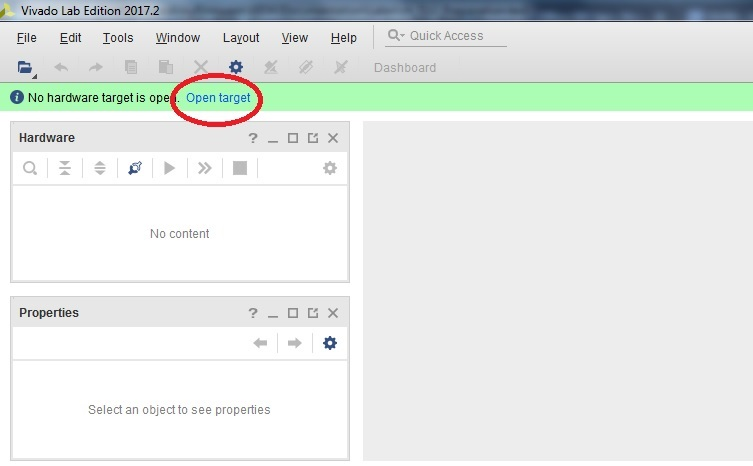
\includegraphics[width=.80\textwidth]{./Images/hw_open.jpg}
  \caption{Vivado interface.}\label{fig:hw_open}
\end{figure}
\begin{figure}
  \centering
  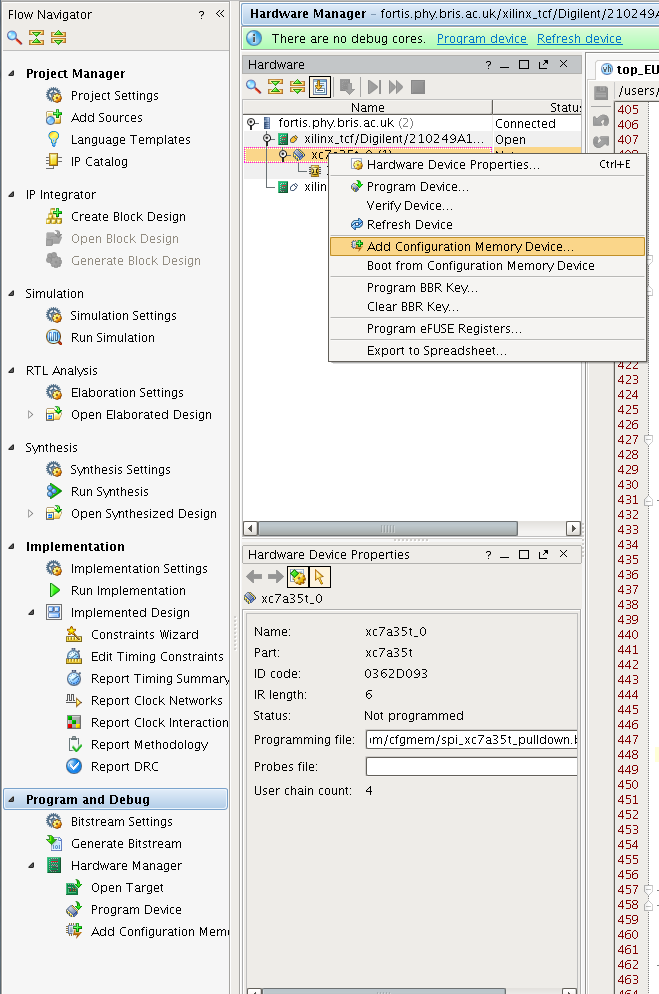
\includegraphics[width=.80\textwidth]{./Images/AddMemory.png}
  \caption{Program interface.}\label{fig:hw_addMemory}
\end{figure}

\subsection{Configuration memory programming}
The procedure to write a permanent program in the \gls{eeprom} is very similar to the one followed to write a bit stream file, with the exception that the user should select \verb"Add configuration memory device" in the options, as shown in figure~\ref{fig:hw_addMemory}.
This will open a new window, shown in figure~\ref{fig:hw_eeprom}, from which it is possible to indicate the file to use (with extension \verb".mcr").
\begin{figure}
  \centering
  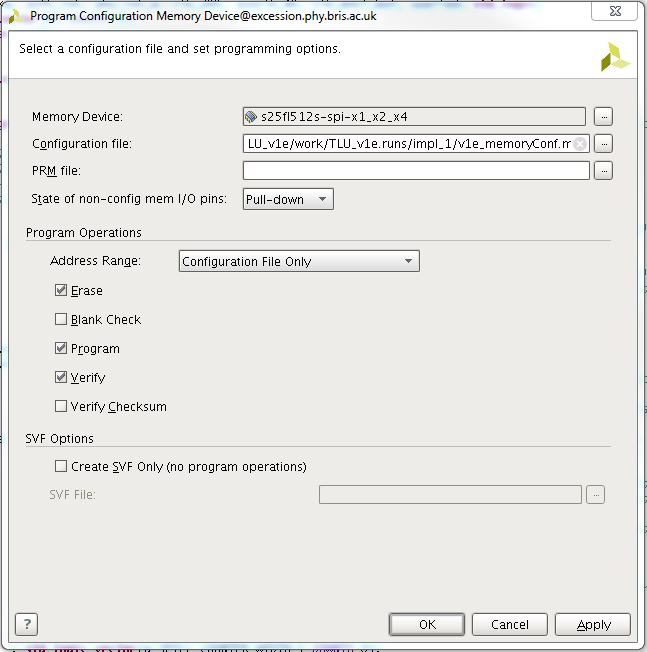
\includegraphics[width=.80\textwidth]{./Images/hw_prog.png}
  \caption{\gls{eeprom} interface. The options shown in the picture are suitable to configure the device correctly.}
  \label{fig:hw_eeprom}
\end{figure}
Make sure that the options are set as shown in figure~\ref{fig:hw_eeprom}.

\section{Inspection}\label{ch:inspection}
At some point someone, somewhere, will want to disassemble the unit to poke at its internal electronics; the top cover of the unit can only slide away when either the front or back frame are removed.
\begin{alertinfo}{Note}
    Simply removing the corner screws on the panels will only allow to remove the plates but not accessing the inside of the unit.
\end{alertinfo}
The frames are held in place by 4 screws hidden behind the corner covers.\\Figure~\ref{fig:dismantle} shows the correct procedure to remove the cover:\\
A) the easiest way to remove the cover is by removing the back frame, rather than the front one.\\
B) Do not remove the corner screws in the plate.\\
C) Remove the two corner covers from the frame. They are only held in place by pressure and can be removed pulling by hand. Once done, remove the 4 Philips screws located behind (green circles).\\
D) unscrew the Philips screw at the bottom of the unit holding the frame in place.\\
E) remove the frame and the back panel. Be careful to not damage the cables connecting the panel to the electronics.\\
F) Slide the top cover away.\\
The same procedure can be repeated with the front frame, if necessary. In this case, the user must also disconnect the front panel from the electronics by removing the countersunk screws connected to the \gls{hdmi} ports and the powermodule.
\begin{figure}
\centering
    \subfloat[A]{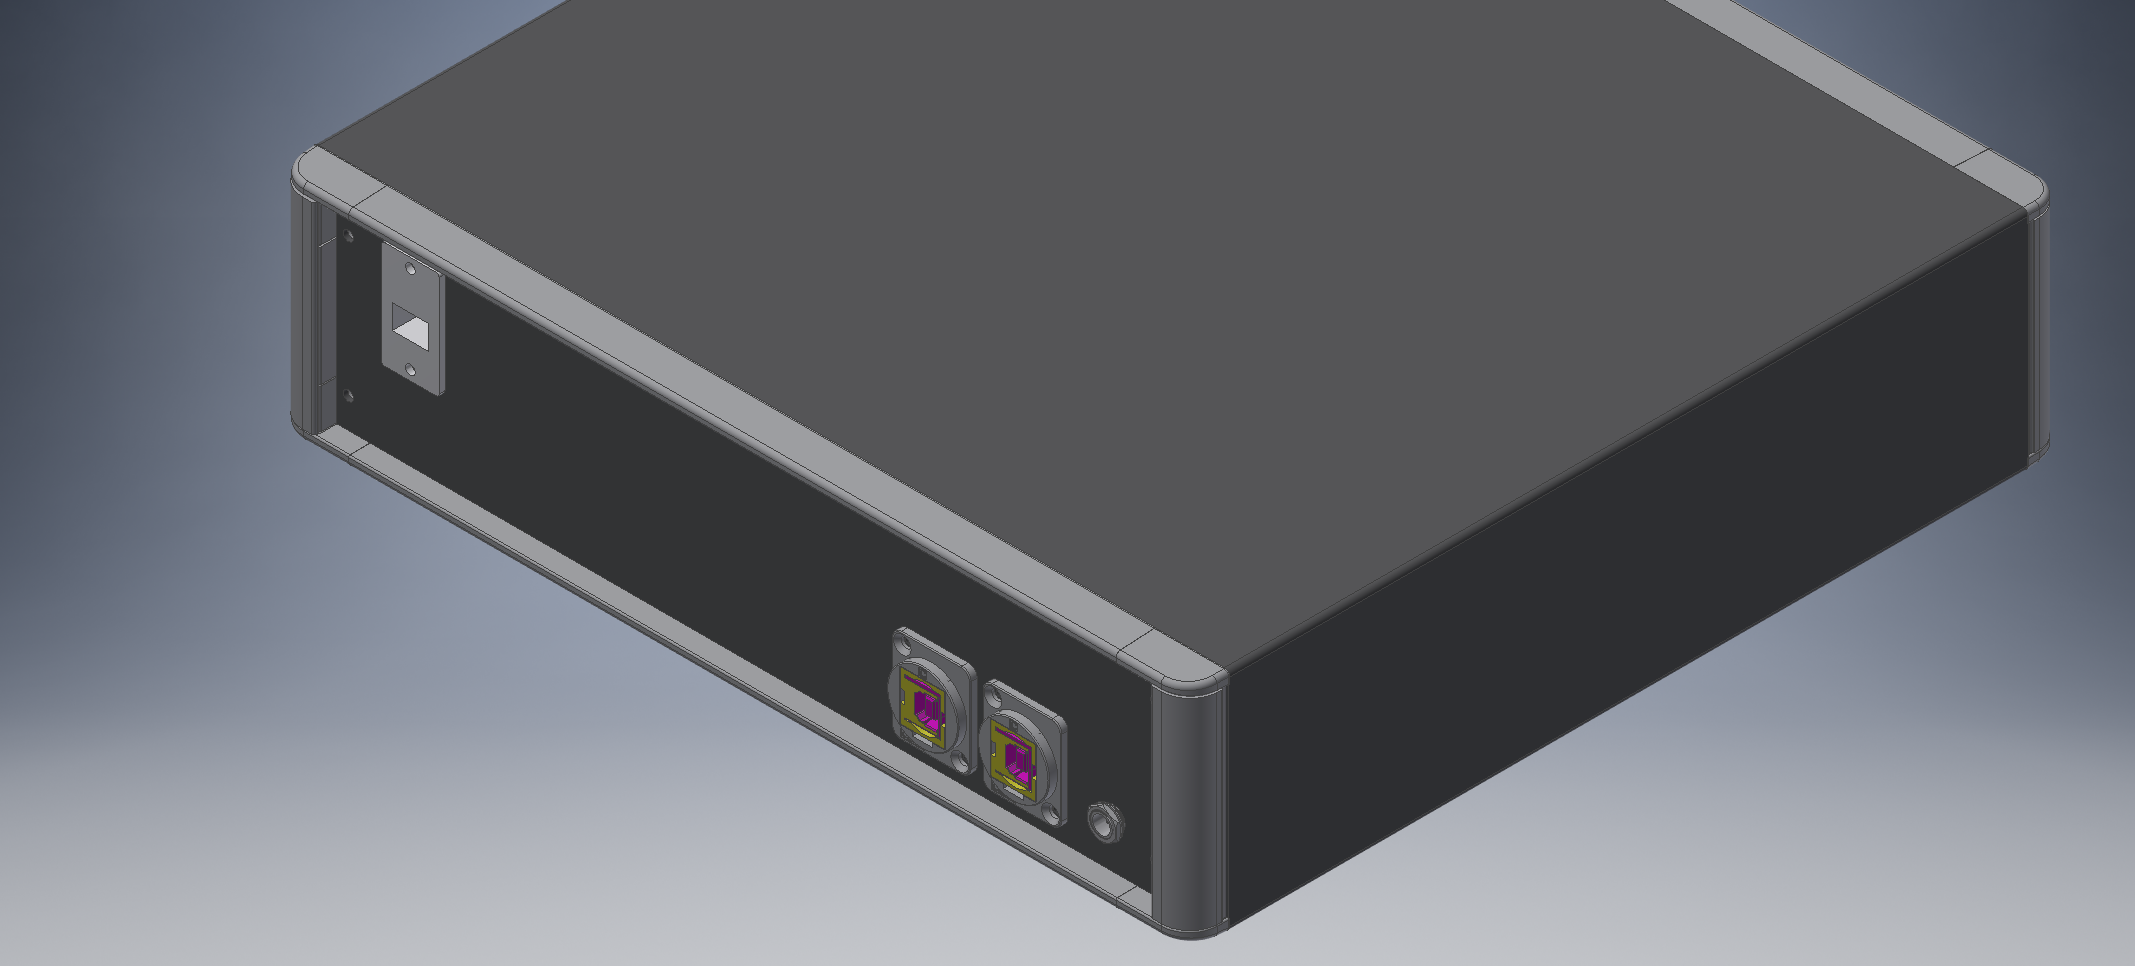
\includegraphics[width=.45\textwidth]{./Images/View1.png}}\hfil
    \subfloat[B]{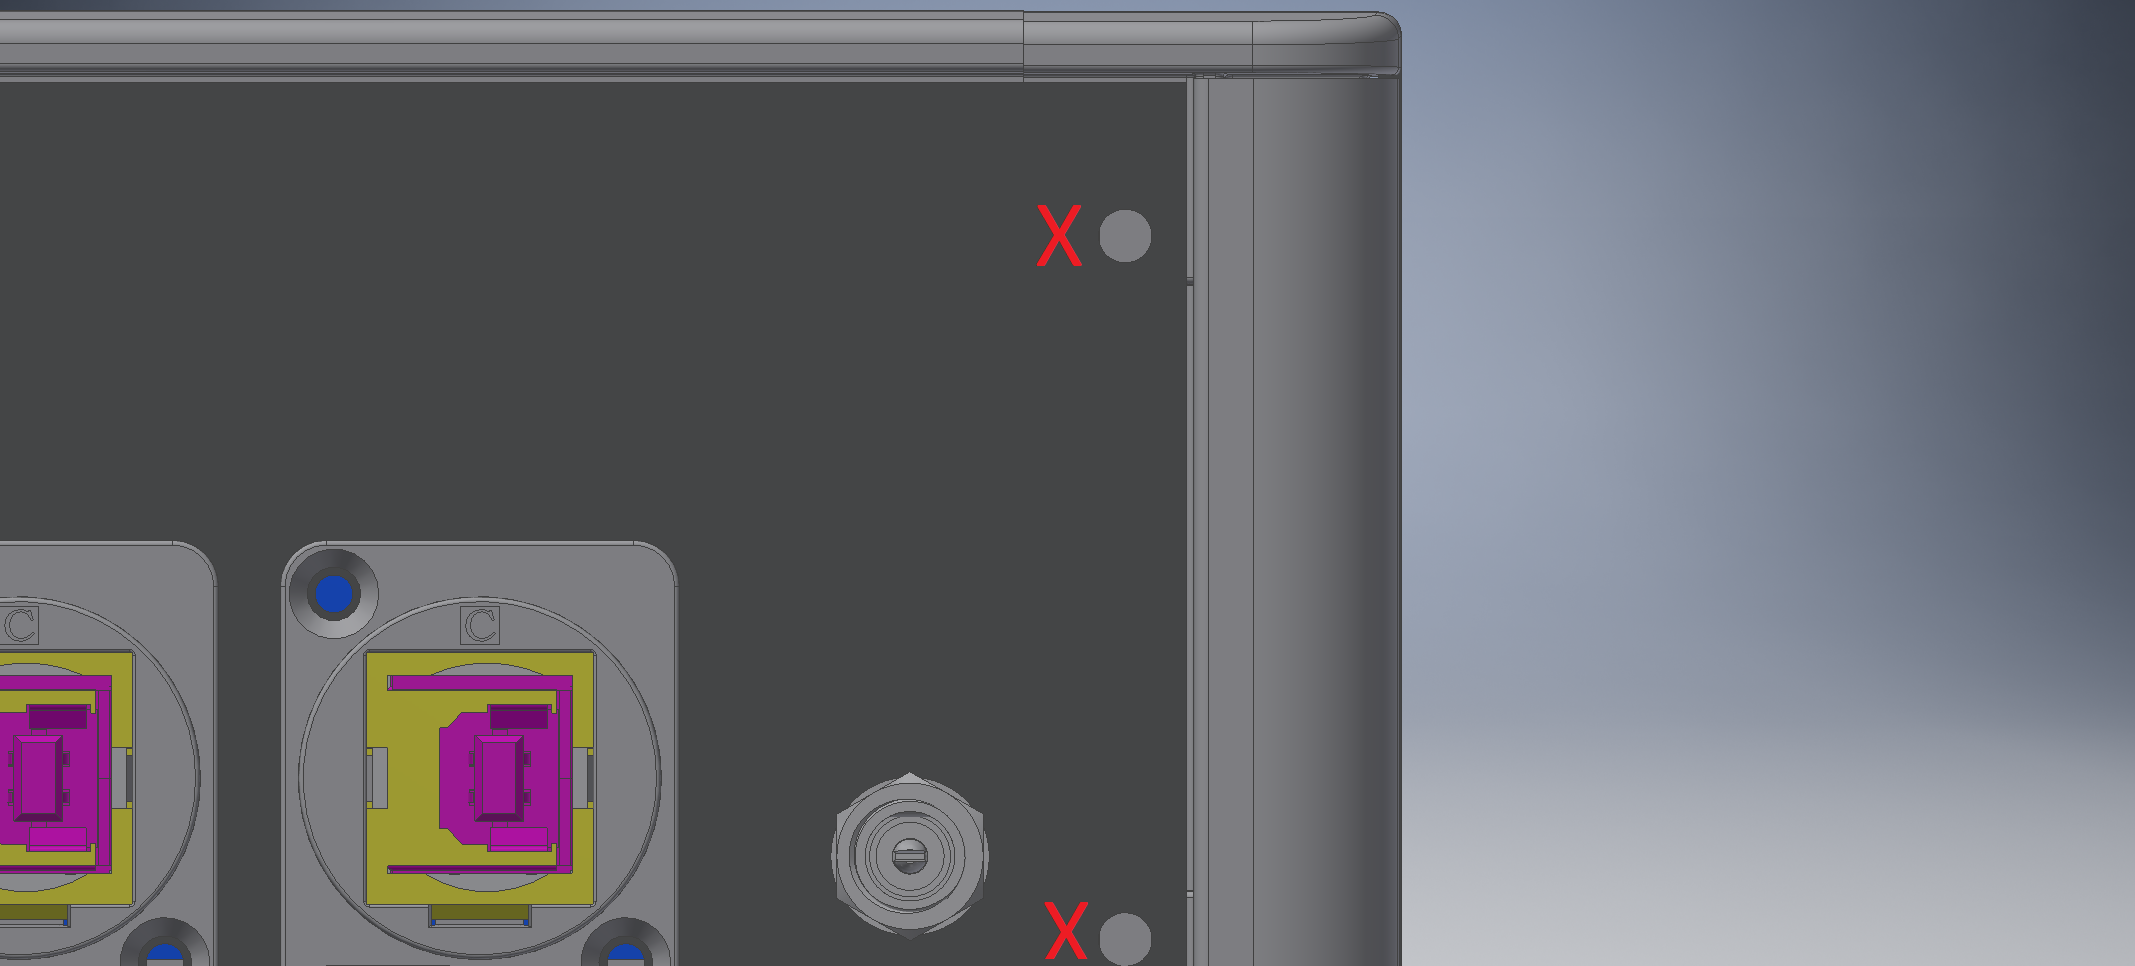
\includegraphics[width=.45\textwidth]{./Images/View6.png}}
    \subfloat[C]{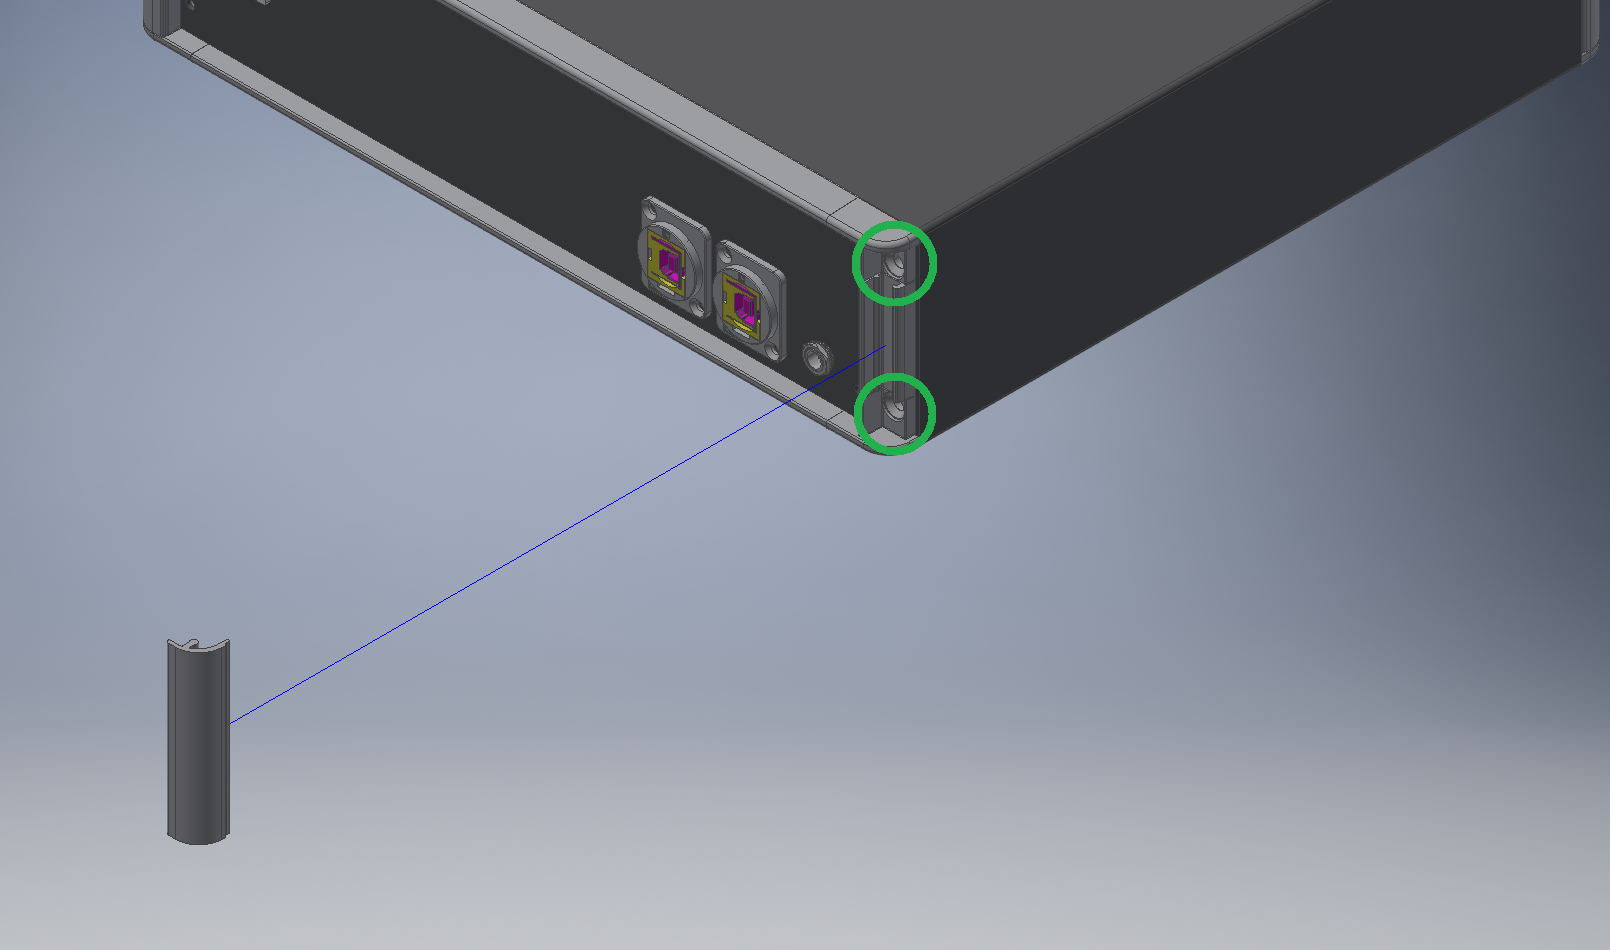
\includegraphics[width=.45\textwidth]{./Images/View2.png}}\hfil
    \subfloat[D]{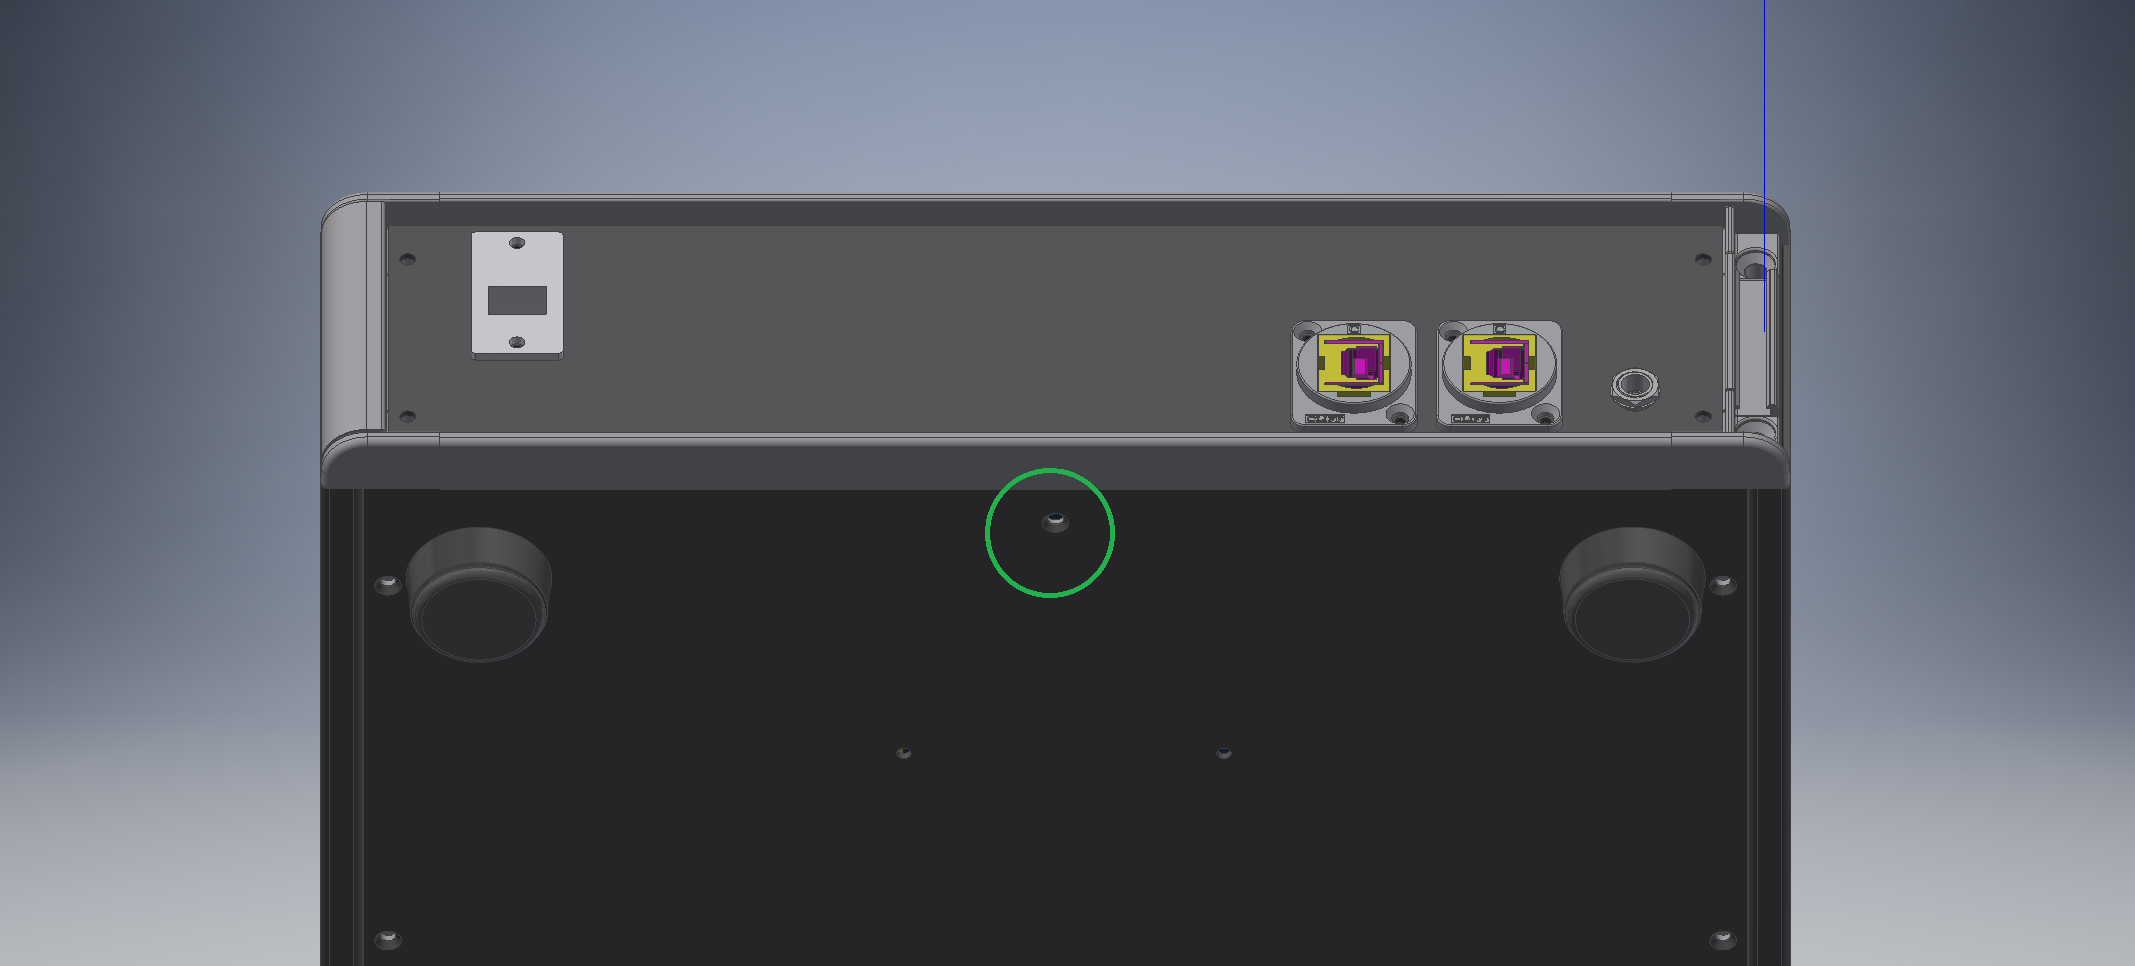
\includegraphics[width=.45\textwidth]{./Images/View3.png}}
    \subfloat[E]{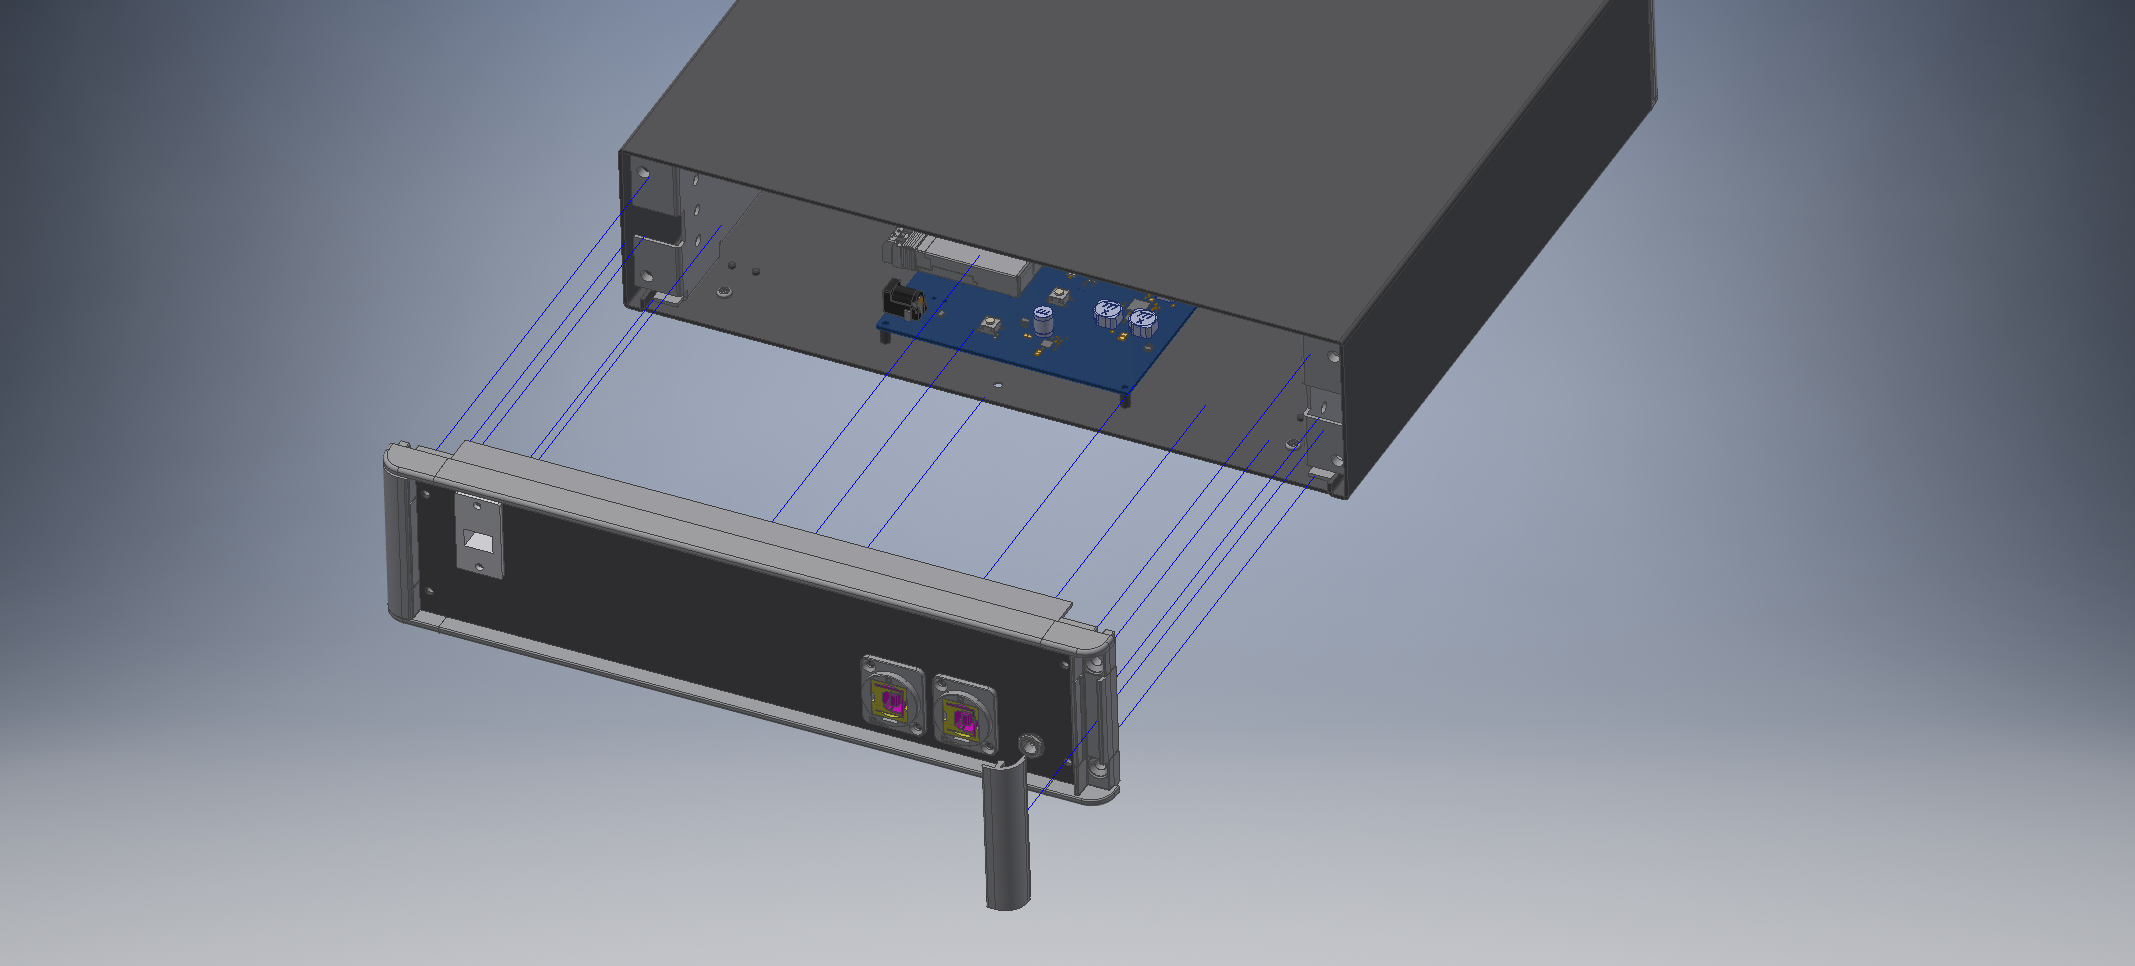
\includegraphics[width=.45\textwidth]{./Images/View4.png}}\hfil
    \subfloat[F]{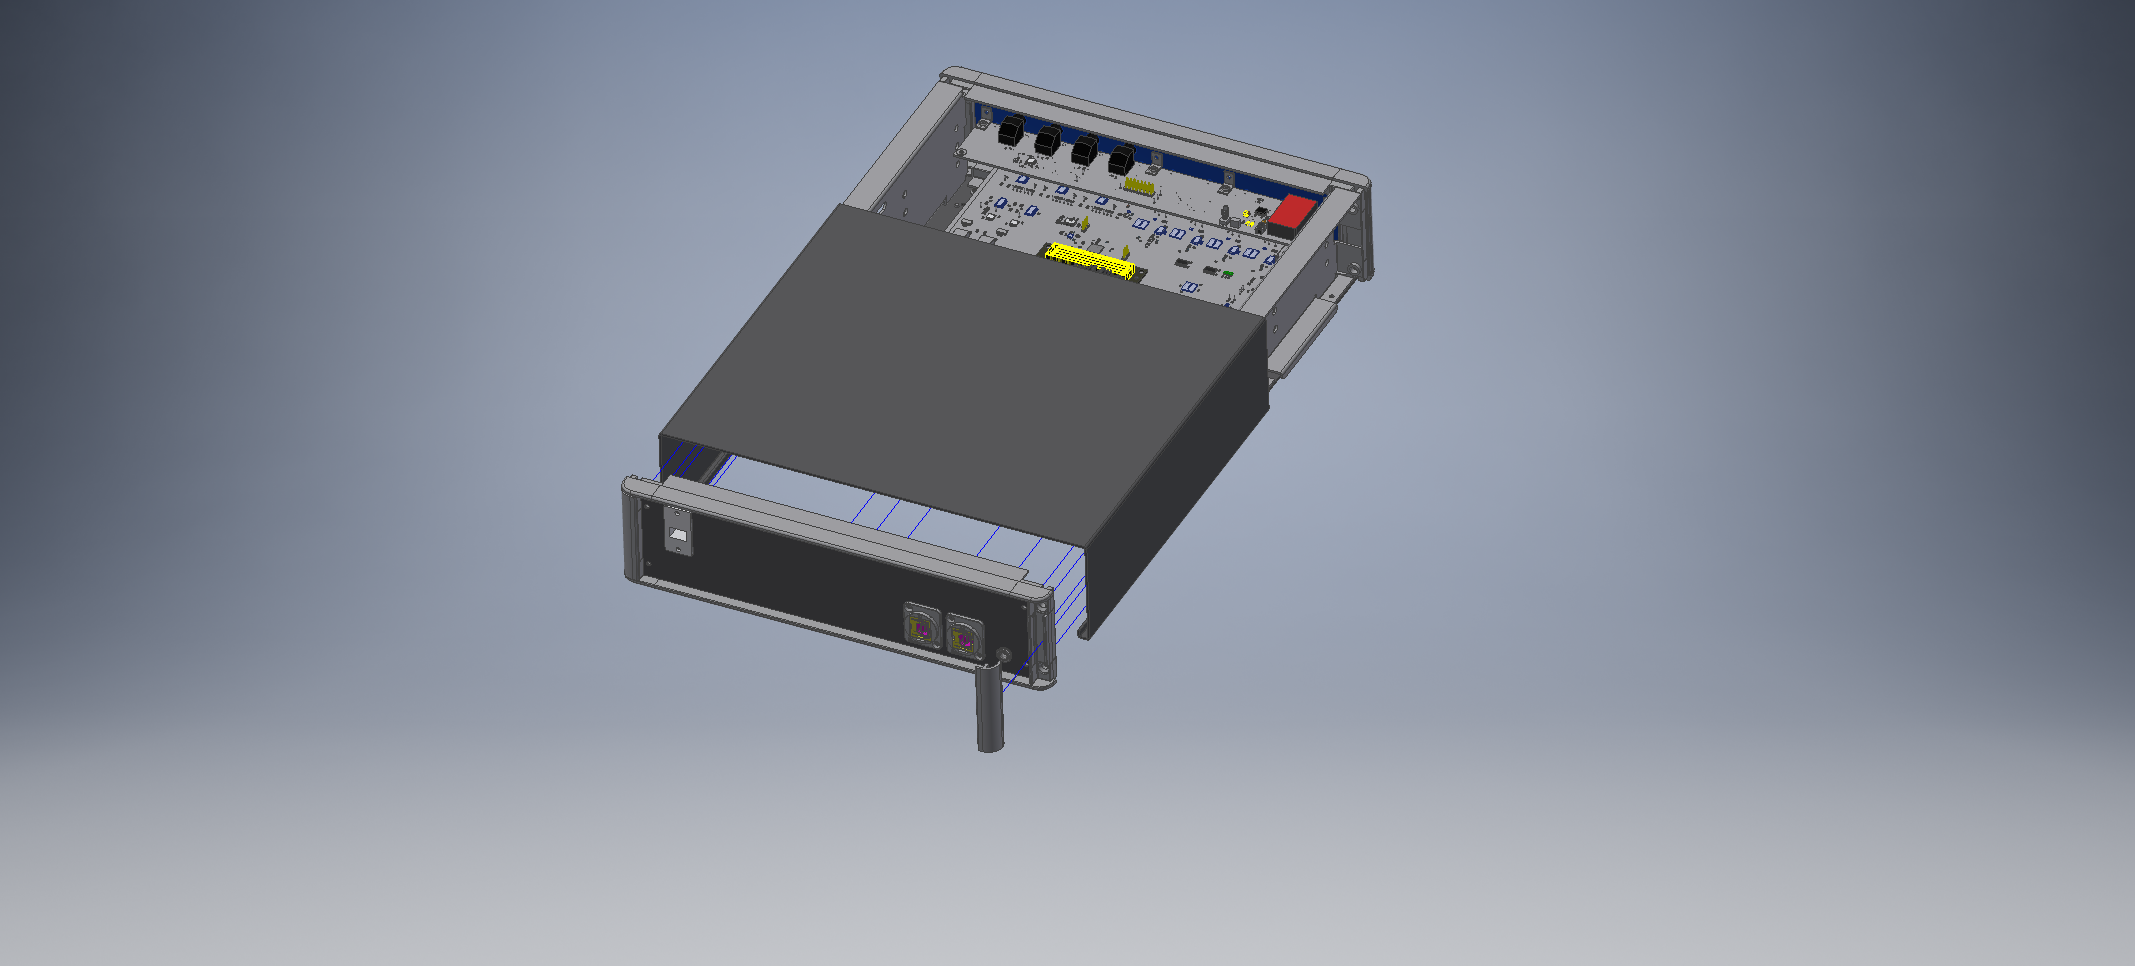
\includegraphics[width=.45\textwidth]{./Images/View5.png}}
    \caption{Steps to remove the cover from the unit.}
    \label{fig:dismantle}
\end{figure}
%\section{Preparation}
%Before powering the \gls{tlu} it is necessary to follow a few steps to ensure the board and the \gls{fpga} work correctly.\\
%
%Currently, it is recommended to use the following:
%\begin{itemize}
% \item MA-PM3-W-R5: Mars PM3 base board
% \item MA-AX3-35-1I-D8-R3: Marx AX3 module (hosts a Xilinx XC7A35T-1CSG324I )
% \item MA-PM3-ACC-BASE: Accessory kit, including a \gls{jtag} breakout board to connect Xilinx programming cables. Also includes a 12~V power supply to power the PM3.
%\end{itemize}
%
%\section{I/O voltage setting}
%The I/O pins of the PM3 can be configured to operate at 2.5~V or 3.3~V; the factory default is 2.5~V but the \brd requires 3.3~V logic. The user should make sure to select the appropriate voltage by operating on DIP-switch CFG-A/S1200 (pin 1 set to ON).\\For reference, a top view of the board is provided in the appendix at page~\pageref{ch:appendix}.\\
%\begin{alertinfo}{Warning}
%    Please double check the PM3 board manual for the correct way to change the I/O voltage setting. Enclustra has been changing their hardware recently.
%\end{alertinfo}
%
%\section{Xilinx programming cable}
%The \gls{jtag} pins on the PM3 are located on the header J800 (20-way, 2.54~mm pitch). The breakout board provided by Enclustra sits on top of the header and connects the pins to a 14-way Molex milli-grid header so that it is possible to plug the Xiling programming cable directly onto it. However, when the \brd is mounted on a base plate as shown in figure~\ref{fig:TLUplate}, the breakout board has to be detached from the PM3 because it interferes with the mounting screws.\\
%The connection between J800 and the breakout can be achieved by using two standard 20-way \gls{idc} cables as shown in figure~\ref{fig:XilinxCable}.
%\begin{figure}[h]
%  \centering
%  \includegraphics[width=.50\textwidth]{./Images/TLU_plate.jpg}
%  \caption{\brd and PM3 mounted on a base plate: in this configuration it is not possible to install the breakout board on the PM3 because the mountings screws are in the way.}\label{fig:TLUplate}
%\end{figure}
%\begin{figure}
%  \centering
%  \includegraphics[width=.80\textwidth]{./Images/XilinxCable.jpg}
%  \caption{Connecting the Xilinx programming cable to the PM3 in an ugly (but effective) way.}\label{fig:XilinxCable}
%\end{figure}
